\documentclass[12pt,fleqn]{article}\usepackage{../../common}
\begin{document}
Green'in Teorisi, Uzaklaşım, Stokes, Yol ve Çizgi Entegralleri

Yüzeyler (Surfaces)

Üç boyut içindeki iki boyut yüzeyler parametrize edilerek gösterilir,
tek boyutlu eğri bir parametre $t$ ile parametrize ediliyordu, alan için
iki değişken $u,v$ gerekir. Notasyonel olarak $r$'nin taradığı bir yüzey

$$
r(u,v) = < x(u,v), y(u,v), z(u,v) >
$$

Mesela $r(u,v) = < u, u^2, v >$ bir yüzey olabilir.

Yüzey alan hesabı için tüm yüzeyi kenarları $\Delta u$, $\Delta v$ olan hücreler
yaratabiliriz. Her noktada iki tane teğet vektör bulunabilir, bunlar $t_u$ ve
$t_v$ olsun,

$$
t_u = < \frac{\partial x}{\partial u},
        \frac{\partial y}{\partial u},
        \frac{\partial z}{\partial u} >, \quad
t_v = < \frac{\partial x}{\partial v},
        \frac{\partial y}{\partial v},
        \frac{\partial z}{\partial v} >        
$$

Yaklaşık olarak her hücrenin alanı $\Delta S_{ij}$ her hücredeki $t_u$ ve $t_v$
(ya da yeni notasyonla onlara $t_u^{ij}$ ve $t_v^{ij}$ diyelim) yönündeki
$\Delta u$ ve $\Delta v$'nin oluşturduğu paralelogram alanıdır, bu paralelogram
bildiğimiz gibi iki vektörün çapraz çarpımından gelen üçüncü vektörün
büyüklüğüdür, o zaman 

$$
\Delta S_{ij} \approx || \Delta u t_u^{ij} \times \Delta v t_v^{ij} ||
$$

$$
= ||  t_u^{ij} \times t_v^{ij} || \Delta u \Delta v
$$
        
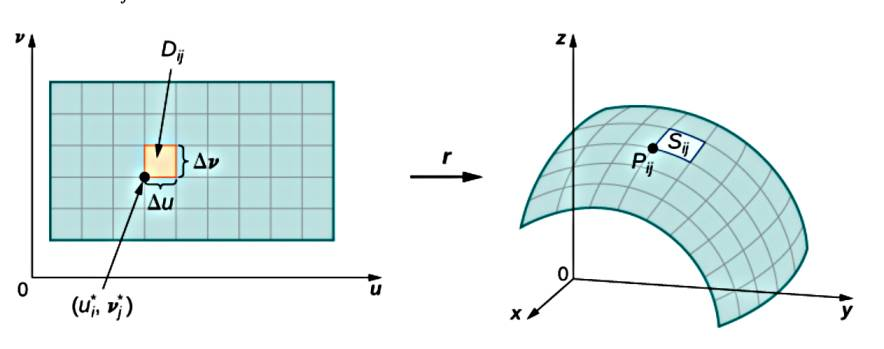
\includegraphics[width=20em]{calc_multi_75_app_01.jpg}

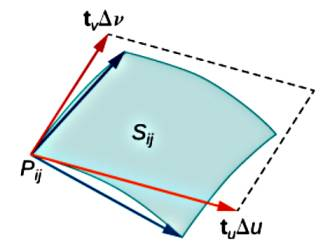
\includegraphics[width=10em]{calc_multi_75_app_02.jpg}

Tüm ufak hücre alanlarını toplarız, ve hücre sayısı sonsuza yaklaşırken toplam
alan limitine bakabiliriz,

$$
\lim_{m,n \to \infty} \sum_{i=1}^{m} \sum_{j=1}^{n} || t_u^{ij} \times t_v^{ij} || \Delta u \Delta v
$$

Bu limit yüzey alan çift entegral hesabına yaklaşır / onu tanımlar, [2, sf. 769],

$$
= \iint_D || t_u \times t_v || \ud u \ud v = \iint_D || t_u \times t_v || \ud A
$$

Yüzey Entegrali (Surface Integral)

Yukarıda gördüklerimiz parametrize edilmiş yüzeyin alanını hesaplamak içindir.
Yüzey entegrali bir yüzey {\em üzerinden} alınan entegrallere verilen isimdir,
mesela tek sayı / skalar değerli bir fonksiyon $f$'nin pürüzsüz bir yüzey $S$
üzerinden alınan yüzey entegrali, o fonksiyonun her noktadaki alan büyüklüğü ile
çarpılıp sonuçların toplanmasıdır, cebirsel olarak yine $t_u,t_v$ kavramlarını
kullanırsak,

$$
\iint_S f(x,y,z) \ud S 
= \lim_{m,n \to \infty} \sum_{i=1}^{m} \sum_{j=1}^{n} f(P_{ij}) || t_u^{ij} \times t_v^{ij} || \Delta u \Delta v
$$

$$
= \lim_{m,n \to \infty} \sum_{i=1}^{m} \sum_{j=1}^{n} f(P_{ij}) \Delta S_{ij} 
$$

O zaman yüzey entegralleri alttaki şekilde hesaplanabilir,

$$
\iint_S f(x,y,z) \ud S =
\iint_D f(r(u,v)) || t_u \times t_v || \ud A
$$

Çizgi entegrali (line integrals) daha düşük boyuttaki benzer bir kavram idi.

Vektör Alanları Üzerinden Yüzey Entegrali

Skalar fonksiyona benzer şekilde bir vektör alanı $F$ ve yüzey $S$ üzerinden de
entegral hesaplanabilir. Yine bir ufak çarpımlar toplamından bahsediyoruz, bu
tür bir hesap pek çok uygulama için faydalı olabilir. Mesela bir su akışı
içindeki geçirgen bir yüzeyi düşünürsek, kütle akışını (mass flux) nasıl
hesaplarız? 

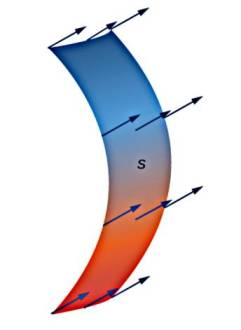
\includegraphics[width=10em]{calc_multi_75_app_04.jpg}

Her noktada yüzey $S$'ye dik olan alan $N$ olsun, her noktadaki akış hızı $v$
diyelim, o zaman bir noktadaki birim zaman ve birim alandaki kütle akışı $\rho v
\cdot N$. Ölçüm birimlerini kontrol edelim, hız $m/s$, yoğunluk $\rho$ 
$g/m^3$, çarparsak $g/s \cdot m^2$ elde ederiz, yani birim alan ve zamandaki
kütle akışı.

Şimdi $\rho v \cdot N$ değerini $\Delta S_{ij}$ ile çarparsak $S$ üzerindeki
hayali ufak hücreden birim zamanda akan kütleyi buluruz, tüm bu akışları
toplarız,

$$
\sum_{i=1}^{m} \sum_{j=1}^{n} (\rho v \cdot N) \Delta S_{ij}
$$

Tüm akışı elde etmiş oluruz. Izgara hücreleri $S_{ij}$ ufaldıkça üstteki toplam
gerçek kütle akışına yaklaşır, yani

$$
\iint_S \rho v \cdot N \ud S = \lim_{m,n \to \infty}
\sum_{i=1}^{m} \sum_{j=1}^{n} (\rho v \cdot N) \Delta S_{ij}
$$

Devam edelim $\rho v$ yerine herhangi bir vektör alanı $F$ kullanalım, o zaman
şu genel tanımı artık yapabiliriz, $F$'nin $S$ yüzeyi üzerinden entegrali

$$
\iint_S \vec{F} \cdot \ud \vec{S} = \iint_S \vec{F} \cdot \vec{N} \ud S
$$

olarak gösterilir.

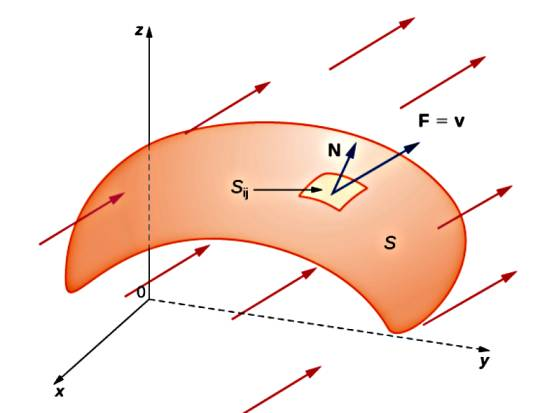
\includegraphics[width=15em]{calc_multi_75_app_05.jpg}

Dikkat her yerde vektör notasyonu kullanmıyoruz, olmadığı yerde formül
çerçevesine göre anlaşılabilir.

$N$ yüzey normalı, öne dik olan birim vektör, hesabı için önceden gördüğümüz
$t_u,t_v$ vektörlerini kullanabiliriz,

$$
N = \frac{t_u \times t_v}{ || t_u \times t_v || }
$$

Üstteki ifadeyi yüzey entegralinde kullanırsak [2, sf. 778],

$$
\iint_S \vec{F} \cdot \vec{N} \ud S =
\iint_S \vec{F} \cdot \frac{t_u \times t_v}{ || t_u \times t_v || } \ud S
$$

Daha önce gördük

$$
\ud S = || t_u \times t_v || \ud u \ud v = || t_u \times t_v || \ud A
$$

İki üste geçirince

$$
= \iint_D \vec{F}(r(u,v)) \cdot \frac{t_u \times t_v}{ || t_u \times t_v || }
|| t_u \times t_v || \ud A
$$

Basitleştirme sonrası,

$$
= \iint_D \vec{F}(r(u,v)) \cdot (t_u \times t_v) || t_u \times t_v || \ud A
$$

Soru

$F = < -y, x, 0 >$ olarak veriliyor, $S$ yüzeyi $r(u,v) = < u, v^2 - u, u+v >$.

$\iint_S F \cdot N \ud S$ yüzey entegralini hesaplayın.

Cevap

Teğet vektörler $t_u = < 1, -1, 1 >$, ve $t_v = < 0, 2v, 1 >$.

$t_u \times t_v$ çapraz çarpımı

\begin{minted}[fontsize=\footnotesize]{python}
import sympy

u,v = sympy.symbols('u v')
t_u = sympy.Matrix([[1,-1,1]])
t_v = sympy.Matrix([[0,2*v,1]])
print (t_u.cross(t_v))
\end{minted}

\begin{verbatim}
Matrix([[-2*v - 1, -1, 2*v]])
\end{verbatim}

Yüzey entegral hesabı şöyle hesaplanabilir,

$$
\int _{0}^{4} \int _{0}^{3} F(r(u,v)) \cdot (t_u \times t_v) \ud u \ud v
$$

Verili $F = < -y, x, 0 >$, ve yüzey $r(u,v) = < u, v^2 - u, u+v >$ demiştik,
o zaman 

$$
F(r(u,v)) = < u-v^2, u, 0 > 
$$

olur. Tüm entegral

$$
= \int _{0}^{4} \int _{0}^{3} < u-v^2, u, 0 >  \cdot < -1-2v, -1, 2v >
\ud u \ud v
$$

$$
= \int_{0}^{4} \int_{0}^{3} (2v^3 + v^2 -2uv -2u )
\ud u \ud v
$$

$$
= \int_{0}^{4} [ 2v^3u + v^2u - vu^2 - u^2 ]_{0}^{3} \ud v
$$

$$
= \int_{0}^{4} (6v^3 + 3v^2 - 9v -9 ) \ud v
$$

$$
= \left[ \frac{3v^4}{2} + v^3 - \frac{9v^2}{2} - 9v \right]_{0}^{4}
$$

$$
= 340
$$

\begin{minted}[fontsize=\footnotesize]{python}
from mpl_toolkits.mplot3d import Axes3D
from matplotlib import cm
import numpy as np
fig = plt.figure()
ax = fig.add_subplot(111, projection='3d')
u = np.linspace(0, 3, 100)
v = np.linspace(0, 4, 100)
u,v = np.meshgrid(u,v)

x = u; y = v**2 - u; z = u + v

ax.plot_surface(x, y, z, rstride=4, cstride=4, cmap = cm.copper)
x = np.linspace(0, 3, 5)
y = np.linspace(0, 10, 5)
z = np.linspace(0, 6, 5)

fu = -y; fv = x; fw = z*0

xx,yy,zz = np.meshgrid(x,y,z)
ax.quiver(xx, yy, zz, fu, fv, fw, length=0.2, color = 'red')
ax.view_init(elev=18, azim=-46)
plt.savefig('calc_multi_75_app_03.jpg',quality=30)
\end{minted}

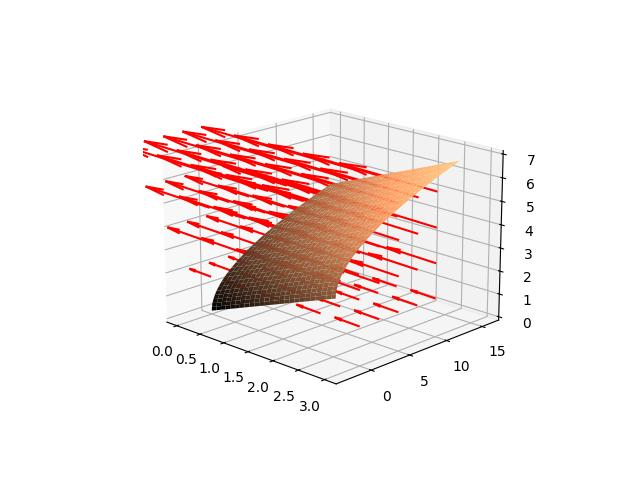
\includegraphics[width=15em]{calc_multi_75_app_03.jpg}














[devam edecek]

Kaynaklar

[1] Marsden, {\em Vector Calculus}

[2] Strang, {\em Calculus Volume 3, OpenStaxa}

\end{document}



